\documentclass[border=7pt]{standalone}
\usepackage{fontspec,unicode-math}
\setmainfont{Noto Serif}
\setmathfont{STIXTwoMath-Regular.otf}
\usepackage{tikz}
\usetikzlibrary{arrows.meta,calc,patterns,decorations.markings,decorations.pathmorphing,decorations.pathreplacing}
\tikzset{lev/.style={line width=1.1pt,line cap=butt},
 fine/.style={line width=.52pt},light/.style={line width=.35pt},
 curve/.style={line width=1.15pt,line cap=round,line join=round},
 ax/.style={line width=.57pt,-{Latex[length=2mm,width=1.15mm]}},
 ray/.style={line width=.58pt,-{Latex[length=1.9mm,width=1mm]},shorten >=1.2pt,shorten <=1.2pt},
 dim/.style={line width=.50pt,{Latex[length=1.65mm,width=.85mm]}-{Latex[length=1.65mm,width=.85mm]}},
 flow/.style={line width=.65pt,postaction={decorate},decoration={markings,mark=at position .6 with {\arrow{Latex[length=1.8mm,width=.95mm]}}}},
 lab/.style={font=\fontsize{12}{14.4}\selectfont,inner sep=1.5pt},
 small/.style={font=\fontsize{10.5}{12.5}\selectfont,inner sep=1.2pt},
 panel/.style={font=\fontsize{12}{14.4}\selectfont\itshape,inner sep=1.5pt}}
\pagestyle{empty}
\begin{document}
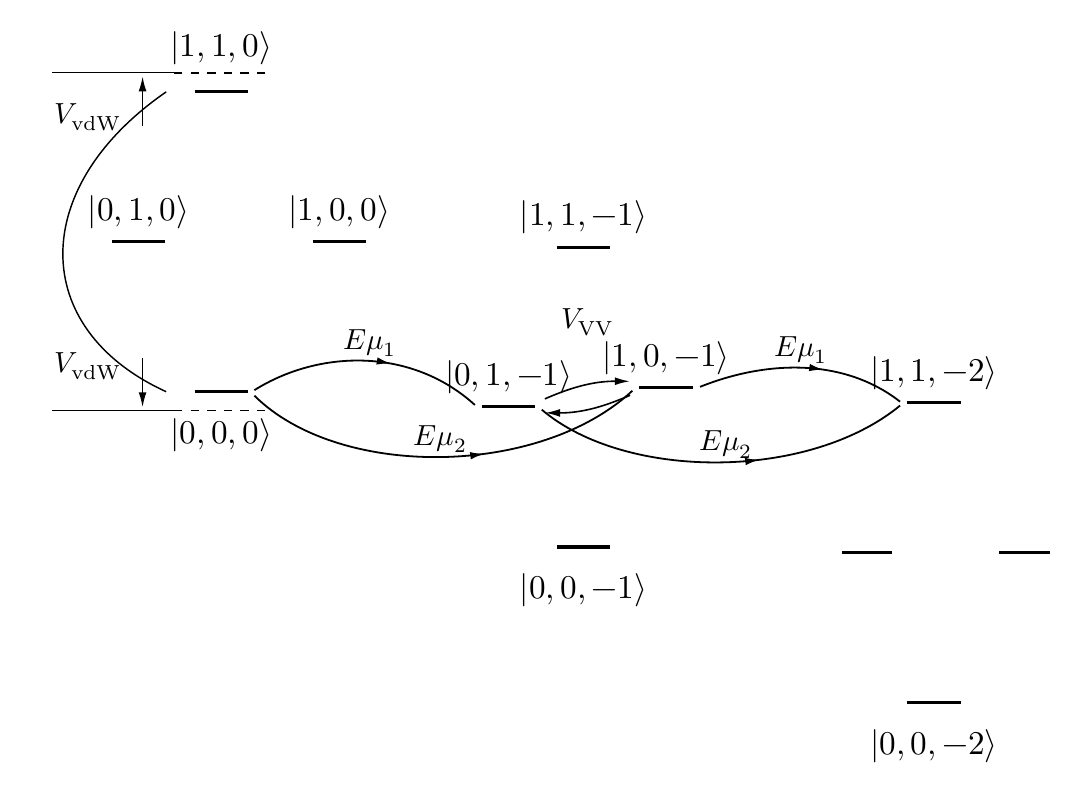
\begin{tikzpicture}[x=1cm,y=1cm,line join=round]
\coordinate (g) at (1.60000,0.00000);\draw[lev] (1.26000,0.00000)--(1.94000,0.00000);
\node[lab,below,yshift=-8pt] at (1.60000,0.00000) {$|0,0,0\rangle$};
\coordinate (ee) at (1.60000,3.80800);\draw[lev] (1.26000,3.80800)--(1.94000,3.80800);
\node[lab,above,yshift=8pt] at (1.60000,3.80800) {$|1,1,0\rangle$};
\coordinate (eg0) at (0.55000,1.90400);\draw[lev] (0.21000,1.90400)--(0.89000,1.90400);
\node[lab,above,yshift=3pt] at (0.55000,1.90400) {$|0,1,0\rangle$};
\coordinate (ge0) at (3.10000,1.90400);\draw[lev] (2.76000,1.90400)--(3.44000,1.90400);
\node[lab,above,yshift=3pt] at (3.10000,1.90400) {$|1,0,0\rangle$};
\coordinate (eem1) at (6.20000,1.83600);\draw[lev] (5.86000,1.83600)--(6.54000,1.83600);
\node[lab,above,yshift=3pt] at (6.20000,1.83600) {$|1,1,-1\rangle$};
% A small schematic splitting separates the two near-resonant intermediate
% levels. No quantitative dipole-dipole coupling is inferred from this gap.
\def\NearSplit{.24}
\coordinate (eg) at (5.25000,-.18800);\draw[lev] (4.91000,-.18800)--(5.59000,-.18800);
\node[lab,above,yshift=3pt] at (5.25000,-.18800) {$|0,1,-1\rangle$};
\coordinate (ge) at (7.25000,.05200);\draw[lev] (6.91000,.05200)--(7.59000,.05200);
\node[lab,above,yshift=3pt] at (7.25000,.05200) {$|1,0,-1\rangle$};
\coordinate (eem2) at (10.65000,-0.13600);\draw[lev] (10.31000,-0.13600)--(10.99000,-0.13600);
\node[lab,above,yshift=3pt] at (10.65000,-0.13600) {$|1,1,-2\rangle$};
\coordinate (gm1) at (6.20000,-1.97200);\draw[lev] (5.86000,-1.97200)--(6.54000,-1.97200);
\node[lab,below,yshift=-8pt] at (6.20000,-1.97200) {$|0,0,-1\rangle$};
\coordinate (gm2) at (10.65000,-3.94400);\draw[lev] (10.31000,-3.94400)--(10.99000,-3.94400);
\node[lab,below,yshift=-8pt] at (10.65000,-3.94400) {$|0,0,-2\rangle$};
\draw[lev] (9.4800,-2.0400)--(10.1200,-2.0400);
\draw[lev] (11.4800,-2.0400)--(12.1200,-2.0400);
\draw[fine,dashed] (1.00000,-0.24000)--(2.18000,-0.24000);
\draw[fine,dashed] (1.00000,4.04800)--(2.18000,4.04800);
\draw[fine] (g) ++(-.7,0) .. controls (-.85,.80) and (-.85,2.6) .. ($(ee)+(-.7,0)$);
\draw[light] (-.55,-0.24000)--(1.0,-0.24000);\draw[ray] (.60,0.47000)--(.60,-0.24000);\node[small,left] at (.38,0.32000) {$V_{\mathrm{vdW}}$};
\draw[light] (-.55,4.04800)--(1.0,4.04800);\draw[ray] (.60,3.33800)--(.60,4.04800);\node[small,left] at (.38,3.48800) {$V_{\mathrm{vdW}}$};

\draw[flow] ($(g)+(.42,.02)$) .. controls (2.85,.54) and (4.02,.56) .. ($(eg)+(-.43,.02)$) node[small,pos=.52,above] {$E\mu_1$};
\draw[flow] ($(g)+(.42,-.05)$) .. controls (3.10,-1.12) and (5.65,-1.08) .. ($(ge)+(-.43,-.04)$) node[small,pos=.50,above] {$E\mu_2$};
\draw[flow] ($(ge)+(.43,.01)$) .. controls (8.55,.41) and (9.52,.42) .. ($(eem2)+(-.43,.01)$) node[small,pos=.48,above] {$E\mu_1$};
\draw[flow] ($(eg)+(.42,-.04)$) .. controls (6.73,-1.13) and (9.06,-1.13) .. ($(eem2)+(-.43,-.04)$) node[small,pos=.52,above] {$E\mu_2$};
\draw[ray] ($(eg)+(.42,.08)$) to[bend left=12] ($(ge)+(-.42,.08)$);
\draw[ray] ($(ge)+(-.42,-.08)$) to[bend left=12] ($(eg)+(.42,-.08)$);
\node[small,fill=white,inner sep=1pt] at (6.25,.88) {$V_{\mathrm{VV}}$};

\end{tikzpicture}
\end{document}
